\documentclass[]{article}
\usepackage{lmodern}
\usepackage{setspace}
\setstretch{2}
\usepackage{amssymb,amsmath}
\usepackage{ifxetex,ifluatex}
\usepackage{fixltx2e} % provides \textsubscript
\ifnum 0\ifxetex 1\fi\ifluatex 1\fi=0 % if pdftex
  \usepackage[T1]{fontenc}
  \usepackage[utf8]{inputenc}
\else % if luatex or xelatex
  \ifxetex
    \usepackage{mathspec}
  \else
    \usepackage{fontspec}
  \fi
  \defaultfontfeatures{Ligatures=TeX,Scale=MatchLowercase}
\fi
% use upquote if available, for straight quotes in verbatim environments
\IfFileExists{upquote.sty}{\usepackage{upquote}}{}
% use microtype if available
\IfFileExists{microtype.sty}{%
\usepackage{microtype}
\UseMicrotypeSet[protrusion]{basicmath} % disable protrusion for tt fonts
}{}
\usepackage[margin = 1in]{geometry}
\usepackage{hyperref}
\hypersetup{unicode=true,
            pdfborder={0 0 0},
            breaklinks=true}
\urlstyle{same}  % don't use monospace font for urls
\usepackage{longtable,booktabs}
\usepackage{graphicx,grffile}
\makeatletter
\def\maxwidth{\ifdim\Gin@nat@width>\linewidth\linewidth\else\Gin@nat@width\fi}
\def\maxheight{\ifdim\Gin@nat@height>\textheight\textheight\else\Gin@nat@height\fi}
\makeatother
% Scale images if necessary, so that they will not overflow the page
% margins by default, and it is still possible to overwrite the defaults
% using explicit options in \includegraphics[width, height, ...]{}
\setkeys{Gin}{width=\maxwidth,height=\maxheight,keepaspectratio}
\IfFileExists{parskip.sty}{%
\usepackage{parskip}
}{% else
\setlength{\parindent}{0pt}
\setlength{\parskip}{6pt plus 2pt minus 1pt}
}
\setlength{\emergencystretch}{3em}  % prevent overfull lines
\providecommand{\tightlist}{%
  \setlength{\itemsep}{0pt}\setlength{\parskip}{0pt}}
\setcounter{secnumdepth}{5}
% Redefines (sub)paragraphs to behave more like sections
\ifx\paragraph\undefined\else
\let\oldparagraph\paragraph
\renewcommand{\paragraph}[1]{\oldparagraph{#1}\mbox{}}
\fi
\ifx\subparagraph\undefined\else
\let\oldsubparagraph\subparagraph
\renewcommand{\subparagraph}[1]{\oldsubparagraph{#1}\mbox{}}
\fi

%%% Use protect on footnotes to avoid problems with footnotes in titles
\let\rmarkdownfootnote\footnote%
\def\footnote{\protect\rmarkdownfootnote}

%%% Change title format to be more compact
\usepackage{titling}

% Create subtitle command for use in maketitle
\providecommand{\subtitle}[1]{
  \posttitle{
    \begin{center}\large#1\end{center}
    }
}

\setlength{\droptitle}{-2em}

  \title{}
    \pretitle{\vspace{\droptitle}}
  \posttitle{}
    \author{}
    \preauthor{}\postauthor{}
    \date{}
    \predate{}\postdate{}
  
\usepackage[left]{lineno}
\linenumbers
\usepackage{caption}

\begin{document}

{
\setcounter{tocdepth}{2}
\tableofcontents
}
Figure 1.
Stylized DateLife workflow. This shows the general worflows and analyses that can be performed with DateLife, via the R package or through the website. Details on the functions involved on each workflow are shown in \texttt{datelife}'s R package vignette.

Figure 2.
Computation time of input processing and search across \texttt{datelife}s chronogram database.

Figure 3.
Lineage through time (LTT) plots of source chronograms containing all or a subset of species from the bird family Fringillidae of true finches. Arrows indicate maximum age of each chronogram. Numbers reference to chronograms' original publications 1: Barker et al. (\protect\hyperlink{ref-barker2012going}{2012}), 2: Barker et al. (\protect\hyperlink{ref-barker2015new}{2015}), 3: Burns et al. (\protect\hyperlink{ref-burns2014phylogenetics}{2014}), 4: Claramunt and Cracraft (\protect\hyperlink{ref-claramunt2015new}{2015}), 5: Gibb et al. (\protect\hyperlink{ref-gibb2015new}{2015}), 6: Hedges et al. (\protect\hyperlink{ref-Hedges2015}{2015}), 7: Hooper and Price (\protect\hyperlink{ref-hooper2017chromosomal}{2017}), 8: Jetz et al. (\protect\hyperlink{ref-Jetz2012}{2012}), 9: Price et al. (\protect\hyperlink{ref-price2014niche}{2014}).

Figure 4.
LTT plots of median and Supermatrix Distance Method (SDM) chronograms summarizing information from source chronograms found for the Fringillidae. Arrows indicate maximum age.

\newpage

\begin{figure}[!h]
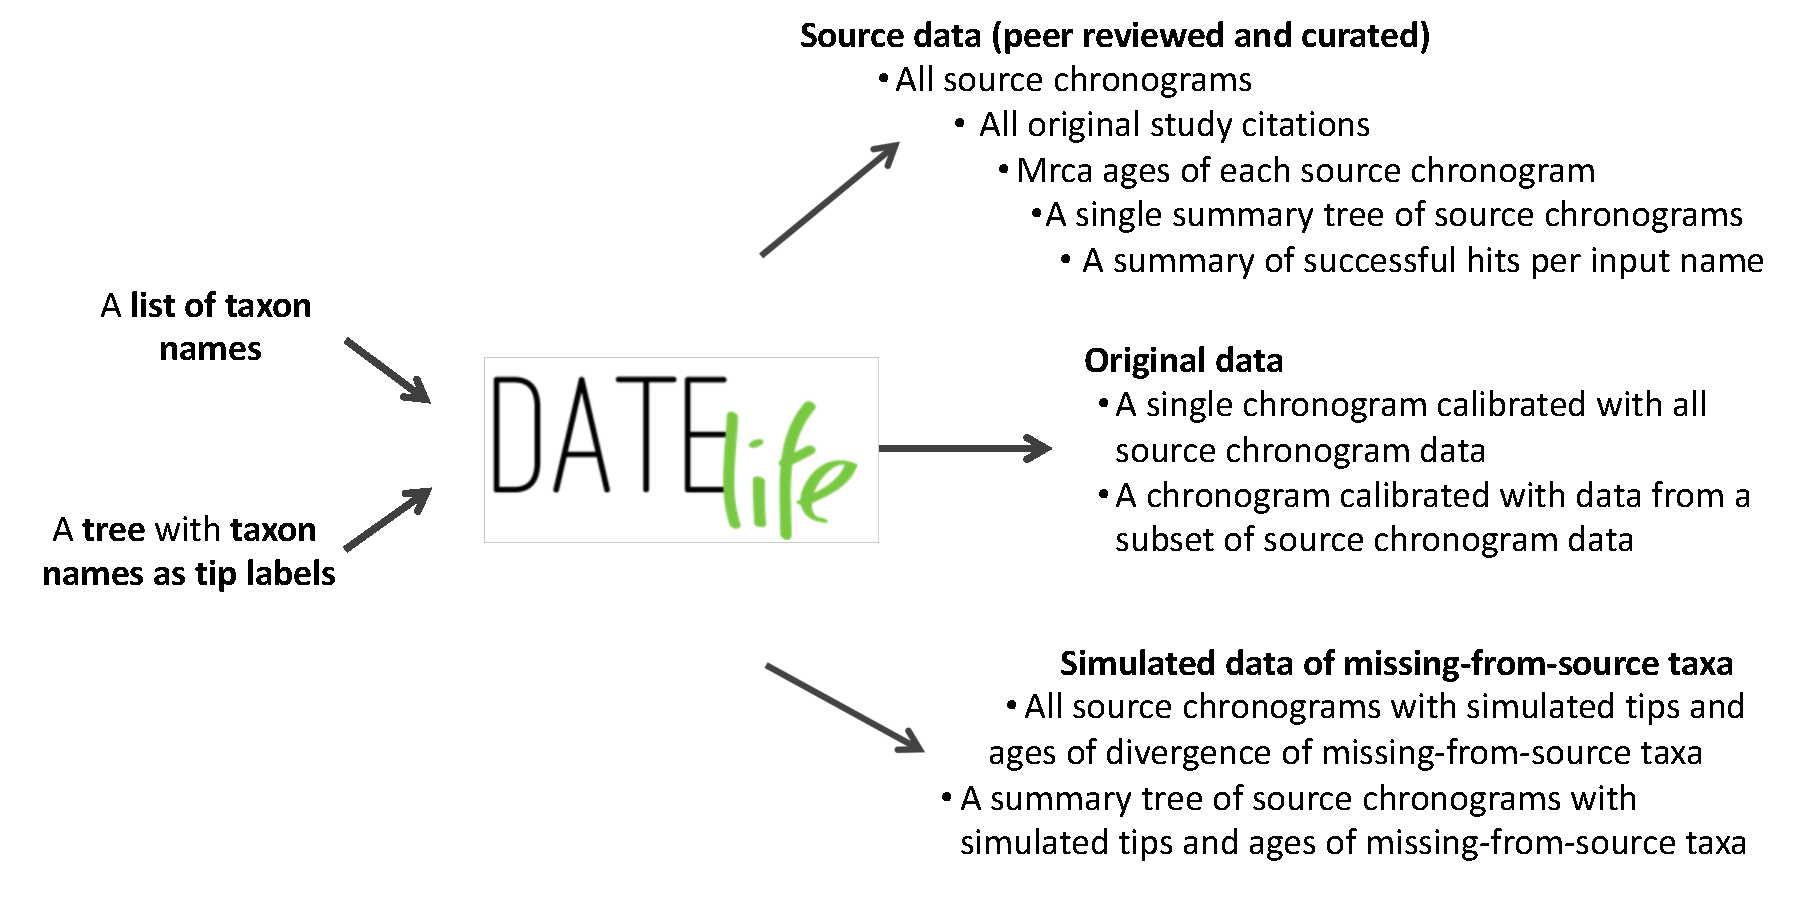
\includegraphics{Fig1.pdf}
\caption{}
\label{fig:workflow}
\end{figure}

\newpage

\begin{figure}[!h]
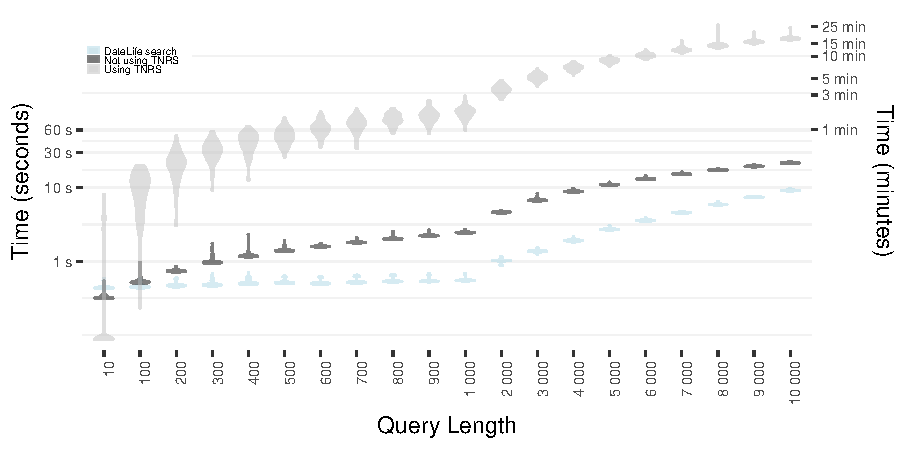
\includegraphics[width=1\linewidth]{fig_runtime1.pdf}
\caption{}
\label{fig:runtime1}
\end{figure}

\newpage

\begin{figure}[!h]
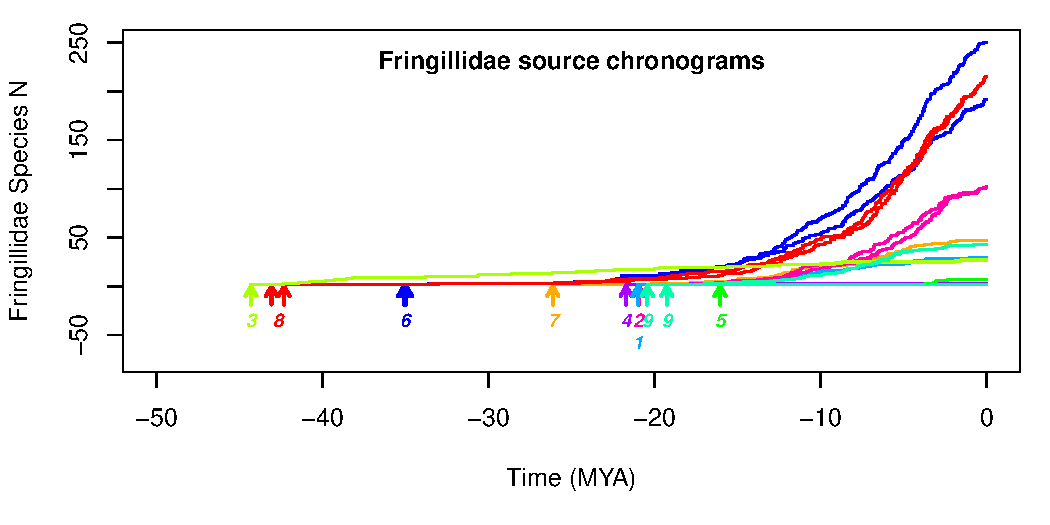
\includegraphics[width=1\linewidth]{fig_schronograms1.pdf}
\caption{}
\label{fig:schronograms}
\end{figure}

\newpage

\begin{figure}[!ht]
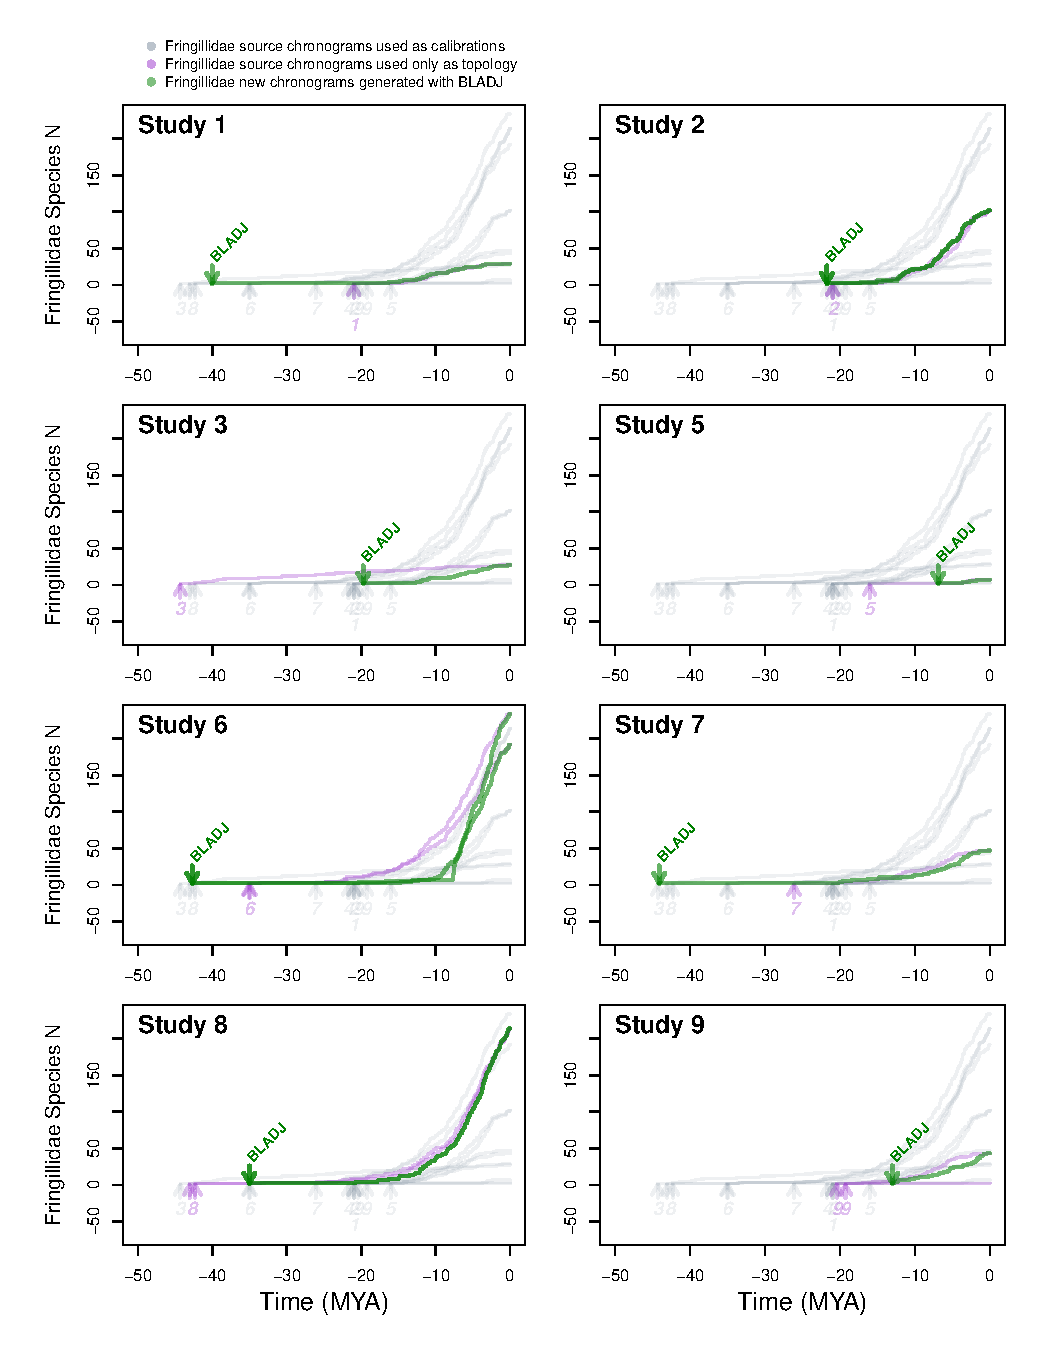
\includegraphics{fig_crossval_bladj.pdf}
\caption{}
\label{fig:cvbladj}
\end{figure}

\hypertarget{refs}{}
\leavevmode\hypertarget{ref-barker2012going}{}%
Barker F.K., Burns K.J., Klicka J., Lanyon S.M., Lovette I.J. 2012. Going to extremes: Contrasting rates of diversification in a recent radiation of new world passerine birds. Systematic biology. 62:298--320.

\leavevmode\hypertarget{ref-barker2015new}{}%
Barker F.K., Burns K.J., Klicka J., Lanyon S.M., Lovette I.J. 2015. New insights into new world biogeography: An integrated view from the phylogeny of blackbirds, cardinals, sparrows, tanagers, warblers, and allies. The Auk: Ornithological Advances. 132:333--348.

\leavevmode\hypertarget{ref-burns2014phylogenetics}{}%
Burns K.J., Shultz A.J., Title P.O., Mason N.A., Barker F.K., Klicka J., Lanyon S.M., Lovette I.J. 2014. Phylogenetics and diversification of tanagers (passeriformes: Thraupidae), the largest radiation of neotropical songbirds. Molecular Phylogenetics and Evolution. 75:41--77.

\leavevmode\hypertarget{ref-claramunt2015new}{}%
Claramunt S., Cracraft J. 2015. A new time tree reveals earth history's imprint on the evolution of modern birds. Science advances. 1:e1501005.

\leavevmode\hypertarget{ref-gibb2015new}{}%
Gibb G.C., England R., Hartig G., McLenachan P.A., Taylor Smith B.L., McComish B.J., Cooper A., Penny D. 2015. New zealand passerines help clarify the diversification of major songbird lineages during the oligocene. Genome biology and evolution. 7:2983--2995.

\leavevmode\hypertarget{ref-Hedges2015}{}%
Hedges S.B., Marin J., Suleski M., Paymer M., Kumar S. 2015. Tree of life reveals clock-like speciation and diversification. Molecular Biology and Evolution. 32:835--845.

\leavevmode\hypertarget{ref-hooper2017chromosomal}{}%
Hooper D.M., Price T.D. 2017. Chromosomal inversion differences correlate with range overlap in passerine birds. Nature ecology \& evolution. 1:1526.

\leavevmode\hypertarget{ref-Jetz2012}{}%
Jetz W., Thomas G., Joy J.J., Hartmann K., Mooers A. 2012. The global diversity of birds in space and time. Nature. 491:444--448.

\leavevmode\hypertarget{ref-price2014niche}{}%
Price T.D., Hooper D.M., Buchanan C.D., Johansson U.S., Tietze D.T., Alström P., Olsson U., Ghosh-Harihar M., Ishtiaq F., Gupta S.K., others. 2014. Niche filling slows the diversification of himalayan songbirds. Nature. 509:222.


\end{document}
